\let\negmedspace\undefined
\let\negthickspace\undefined
\documentclass[journal]{IEEEtran}
\usepackage[a5paper, margin=10mm, onecolumn]{geometry}
%\usepackage{lmodern} % Ensure lmodern is loaded for pdflatex
\usepackage{tfrupee} % Include tfrupee package
\setlength{\headheight}{1cm} % Set the height of the header box
\setlength{\headsep}{0mm}     % Set the distance between the header box and the top of the text
\usepackage{gvv-book}
\usepackage{gvv}
\usepackage{cite}
\usepackage{amsmath,amssymb,amsfonts,amsthm}
\usepackage{algorithmic}
\usepackage{graphicx}
\usepackage{textcomp}
\usepackage{xcolor}
\usepackage{txfonts}
\usepackage{listings}
\usepackage{enumitem}
\usepackage{mathtools}
\usepackage{gensymb}
\usepackage{comment}
\usepackage[breaklinks=true]{hyperref}
\usepackage{tkz-euclide} 
\usepackage{listings}
% \usepackage{gvv}                                        
\def\inputGnumericTable{}                                 
\usepackage[latin1]{inputenc}                                
\usepackage{color}                                            
\usepackage{array}                                            
\usepackage{longtable}                                       
\usepackage{calc}                                             
\usepackage{multirow}                                         
\usepackage{hhline}                                           
\usepackage{ifthen}                                           
\usepackage{lscape}
\renewcommand{\thefigure}{\theenumi}
\renewcommand{\thetable}{\theenumi}
\setlength{\intextsep}{10pt} % Space between text and floats
\numberwithin{equation}{enumi}
\numberwithin{figure}{enumi}
\renewcommand{\thetable}{\theenumi}
\begin{document}
\bibliographystyle{IEEEtran}
\title{Question 9-9.3-3}
\author{EE24BTECH11015 - Dhawal}
% \maketitle
% \newpage
% \bigskip
{\let\newpage\relax\maketitle}
\begin{enumerate}
\item Find the area enclosed by the parabola $4y = 3x^2$ and the line $2y = 3x+12$. 

\end{enumerate}

\begin{table}[h!]    
  \centering
  
\begin{tabular}[12pt]{ |c| c| c|}
    \hline
    \textbf{Variable} & \textbf{Description} & \textbf{Values} \\ 
    \hline
    AB & Length & 6 cm \\
    \hline
    BC & Length & 8 cm \\
    \hline
    $\angle ABC$ & Angle & \ang{60}\\
    \hline 
    $\vec{A}$ & Point & $(6,0)$ \\
    \hline
    $\vec{B}$ & Origin & $(0,0)$ \\
    \hline
    $\vec{C}$ & To find & ? \\
    \hline
    \end{tabular}


  \caption{Variables given}
  \label{tab 1.4.9.2}
\end{table}
Solution:\\
Parabola in terms of matrix:
\begin{align}
\text{g}\brak{\vec{x}}=\vec{x}^{\top}\vec{V}\vec{x}+2\vec{u}^{\top}\vec{x}+f=0
\end{align}
Where:
\begin{align}
\vec{V}=\myvec{3&&0\\0&&0} \hspace{1cm} \vec{u}=\myvec{0\\-2} \hspace{1cm} f=0
\end{align}
Point of intersection of line L
\begin{align}
	L: \quad \vec{x} = \vec{h} + \kappa \vec{m} \quad \kappa \in \mathbb{R}
\end{align}
Where:
\begin{align}
\vec{h}=\myvec{0\\6} \hspace{1cm} \vec{m}=\myvec{1\\\frac{3}{2}}
\end{align}
is represented by:
\begin{align}
	\vec{x}_i = \vec{h} + \kappa_i \vec{m}
\end{align}
Where:
\begin{align}
	\kappa_i = \frac{1}
{
\vec{m}^{\top}\vec{V}\vec{m}
}
\lbrak{-\vec{m}^{\top}\brak{\vec{V}\vec{h}+\vec{u}}}
\pm
\rbrak{\sqrt{
\sbrak{
\vec{m}^{\top}\brak{\vec{V}\vec{h}+\vec{u}}
}^2
	-\text{g}
\brak
{\vec{h}
}
\brak{\vec{m}^{\top}\vec{V}\vec{m}}
}
}
\end{align}
Finding $\text{g}\brak{\vec{h}}$:
\begin{align}
	\text{g}\brak{\vec{h}}=-24
\end{align}
Finding $\kappa_i$:
\begin{align}
	\kappa_i=4 \text{ and } -2
\end{align}
So Points of intersection are:
\begin{align}
	\vec{x}_i=\myvec{4\\12} \text{ and } \myvec{-2\\3}\\
 \vec{A}=\myvec{4\\12} \vec{B}=\myvec{-2\\3}
\end{align}
Area between the curves:
\begin{align}
     \int_{-2}^{4}\brak{1.5x-6-0.75x^2}\,dx =31
\end{align}
So Area between the graphs is 31.\\



Plot:
\begin{figure}[h!]
   \centering
   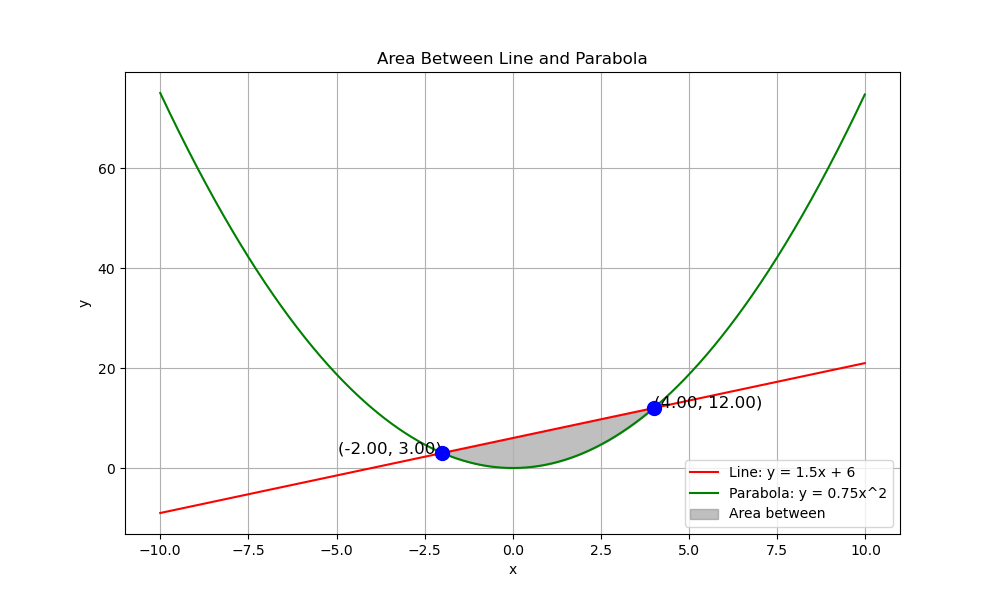
\includegraphics[width=0.9\linewidth]{Figure_1.png}
	\caption{Area Enclosed by parabola and line. }
   \label{stemplot}
\end{figure}


\end{document}

